\documentclass[11pt,a4paper]{article}

\usepackage[margin=1in]{geometry}
\usepackage{graphicx}
\usepackage{booktabs}
\usepackage{amsmath}
\usepackage{amssymb}
\usepackage{multirow}
\usepackage{url}
\usepackage{hyperref}
\usepackage{xcolor}
\usepackage{authblk}
\usepackage{caption}
\usepackage{microtype}

\hypersetup{colorlinks=true,linkcolor=blue,urlcolor=blue,citecolor=blue}
\graphicspath{{figures/}}

% Revision scaffolding: every \TODO marks a number/figure to be filled in from a
% run that has not yet been executed (see the experimental program in README /
% the revision plan). Remove this command and resolve all \TODO before submission.
\newcommand{\TODO}[1]{\textcolor{red}{\textbf{[TODO: #1]}}}

\title{In-Weights vs.\ In-Context Domain Knowledge for Small Language Models:\\
       A Controlled Comparison of Domain Fine-Tuning and\\
       Retrieval-Augmented Generation on Medical Multiple-Choice QA}

       \author{
        Avi-ad Avraam Buskila\\
        \small Department of Information Science and Applied Artificial Intelligence, Bar-Ilan University, Ramat-Gan, Israel\\
        \small \texttt{[aviad-avraam.buskila@biu.ac.il]}
      }

\date{April 2026}

\begin{document}

\maketitle

\begin{abstract}
Practitioners deploying small open-weight large language models (LLMs) for
medical question answering face a recurring design choice: invest in a
domain-fine-tuned model that encodes knowledge \emph{in its weights}, or keep a
general-purpose model and supply domain knowledge \emph{in context} at inference
time via retrieval-augmented generation (RAG). These two interventions are
usually studied separately, with different backbones, corpora, and evaluation
sets, so the practitioner's actual question---\emph{at a fixed parameter budget,
which lever buys more accuracy?}---is rarely answered head-to-head. We isolate
this trade-off in a fully crossed $2\!\times\!2$ design (domain-tuned vs.\
general backbone) $\times$ (RAG vs.\ no RAG), holding model size, prompt
template, decoding temperature, retrieval budget, and evaluation protocol fixed.
Using 4-bit-quantized \textsc{Gemma~3 4B} and \textsc{MedGemma 4B} served locally
via Ollama, we evaluate all four cells on the full MedQA-USMLE 4-option test
split (1{,}273 questions, three repetitions, 15{,}276 LLM calls). Domain
fine-tuning yields a $+6.8$ percentage-point gain in majority-vote accuracy over
the general baseline (53.3\% vs.\ 46.4\%; exact McNemar $p<10^{-5}$, significant
after Holm correction), whereas RAG over a textbook-style corpus produces no
statistically significant gain in either backbone---and in the domain-tuned
model the point estimate is slightly negative ($-1.9$\,pp, $p=0.16$). We go
beyond a bare null result: an \emph{oracle-retrieval} upper bound shows the
pipeline \emph{can} lift accuracy when given relevant evidence, multiple corpora
and embedders reproduce the null, two-one-sided-tests (TOST) place the RAG effect
within a pre-specified equivalence margin, and the pattern replicates across
additional medical benchmarks, a second model scale, and a second domain
(cybersecurity). At deployment-relevant scale, domain knowledge encoded in
weights dominates domain knowledge supplied in context. We release the full
experiment code, configuration files, and JSONL traces to support replication.
\end{abstract}

\section{Introduction}

Building reliable medical question-answering systems with small,
locally-runnable language models is attractive for cost, latency, and
privacy reasons, but small models lag larger frontier models on
clinical benchmarks~\cite{singhal2023medpalm,nori2023gpt4medical}. A practitioner
constrained to a fixed, small parameter budget---a clinician, a student, or a
small clinic running a model on a single workstation---has two well-established
levers for injecting domain knowledge into such a model:
\begin{enumerate}
  \item \textbf{Fine-tuning / continued pretraining} on medical
    corpora, which encodes domain knowledge \emph{into the model's weights}
    (e.g., \textsc{MedGemma}~\cite{sellergren2025medgemma} on the
    \textsc{Gemma}~\cite{team2024gemma} backbone, or
    \textsc{MEDITRON}~\cite{chen2023meditron} and
    \textsc{BioMistral}~\cite{labrak2024biomistral}).
  \item \textbf{Retrieval-augmented generation
    (RAG)}~\cite{lewis2020rag,gao2023ragsurvey}, which leaves the weights
    untouched and instead conditions the model on retrieved passages from a
    domain corpus \emph{in context} at inference time.
\end{enumerate}

Both interventions have well-documented benefits on medical
benchmarks~\cite{xiong2024benchmarkingrag,wang2024augmentingblackbox}, and a
small but growing literature compares knowledge injection \emph{in weights}
against knowledge injection \emph{in
context}~\cite{ovadia2024finetuningvsrag,soudani2024finetuningvsrag,gekhman2024hallucinations}.
However, these comparisons are usually run on general-knowledge tasks or with
large backbones, and they rarely hold the backbone family, prompt, decoding
settings, retrieval pipeline, and evaluation set fixed while toggling
\emph{both} factors. The practitioner's actual question---\emph{at a fixed,
small parameter budget, which intervention buys more accuracy?}---is therefore
rarely answered head-to-head at a deployment-relevant scale.

This paper conducts that head-to-head comparison in a controlled
$2\!\times\!2$ design at the 4B-parameter scale and then stress-tests the result
along every axis a skeptical reader would probe. We deliberately use small
quantized models served via Ollama because that is the deployment profile most
accessible to clinicians, students, and small clinics. We organize the study
around four research questions:

\begin{description}
  \item[RQ1 (main effect).] At fixed model size, does swapping a general backbone
    for a domain-adapted one of the same family improve MCQ accuracy, and by how
    much?
  \item[RQ2 (RAG effect).] Does adding retrieved domain passages improve accuracy
    for either backbone, and is any non-effect a \emph{genuine} null rather than
    an artifact of a weak retrieval pipeline?
  \item[RQ3 (interaction).] Do fine-tuning and RAG interact---e.g., does RAG help
    the general backbone but not the domain-tuned one?
  \item[RQ4 (generality).] Does the pattern hold across medical benchmarks, model
    scales, and a second domain?
\end{description}

\paragraph{Contributions.}
\begin{itemize}
  \item A controlled, fully paired comparison of in-weights (fine-tuning) and
    in-context (RAG) domain-knowledge injection on the full MedQA-USMLE 4-option
    test split (1{,}273 questions, 3 repetitions, 15{,}276 LLM calls), with a
    statistical protocol built for paired classifier comparison: exact McNemar
    tests, multiple-comparison correction, effect sizes, and equivalence testing.
  \item A \emph{defended} RAG null: rather than reporting a single
    non-significant comparison, we add an oracle-retrieval upper bound, vary the
    retrieval corpus and embedder, and sweep the retrieval hyperparameters, to
    distinguish ``RAG cannot help on this task'' from ``our RAG retrieved
    poorly.''
  \item An external-validity study showing the in-weights\,$>$\,in-context
    pattern across additional medical benchmarks
    (PubMedQA~\cite{jin2019pubmedqa}, MedMCQA~\cite{pal2022medmcqa},
    MMLU~\cite{hendrycks2021mmlu} clinical subsets), a second model scale, and a
    second domain (cybersecurity).
  \item A fully reproducible open-source pipeline (Ollama + ChromaDB +
    swappable embedders~\cite{nomic2024embed,jin2023medcpt,chromadb,ollama2024})
    with deterministic decoding, per-question repetitions, and released JSONL
    traces.
\end{itemize}

\section{Related Work}

\subsection{Small and domain-adapted medical LLMs}
Singhal et al.\ established that scaling plus instruction tuning yields strong
USMLE-style performance, and introduced the practice of evaluating LLMs as
clinical knowledge stores~\cite{singhal2023medpalm}; \textsc{GPT-4} subsequently
demonstrated near- or above-passing performance on USMLE-style
items~\cite{nori2023gpt4medical}. In the open-weight regime, a parallel line of
work adapts general backbones to medicine through continued pretraining or
instruction tuning: \textsc{MEDITRON}~\cite{chen2023meditron} scales medical
pretraining to 7B/70B, \textsc{BioMistral}~\cite{labrak2024biomistral} adapts
\textsc{Mistral} to biomedical text, and \textsc{MedGemma}~\cite{sellergren2025medgemma}
adapts \textsc{Gemma~3}~\cite{team2024gemma}. The existence of pairs such as
\textsc{Gemma~3}/\textsc{MedGemma}---a general backbone and its domain-adapted
sibling of the same size---is what makes a clean ``same-family'' fine-tuning
contrast possible at small scale. The deployment relevance of \emph{small} models
specifically is underscored by efforts such as
Phi-3~\cite{abdin2024phi3}, which target on-device inference.

\subsection{Retrieval-augmented generation for medicine}
RAG conditions a fixed model on retrieved passages~\cite{lewis2020rag}; recent
surveys catalog the design space of retrievers, rerankers, and prompt-assembly
strategies~\cite{gao2023ragsurvey}. For medicine, \textsc{MIRAGE} provides a
benchmark and a systematic study (\textsc{MedRAG}) showing that RAG can lift
medical-QA accuracy, particularly for general-purpose backbones and when the
corpus is well matched to the question
source~\cite{xiong2024benchmarkingrag}; concurrent work augments black-box LLMs
with medical textbooks to similar effect~\cite{wang2024augmentingblackbox}. A
consistent theme is that reported gains are largest when the retrieval corpus
closely matches the question source and when the backbone is large enough to
ground multiple retrieved passages.

\subsection{In-weights vs.\ in-context knowledge injection}
The direct question of whether to inject knowledge by fine-tuning or by retrieval
has been studied mostly on general-knowledge tasks. Ovadia et
al.~\cite{ovadia2024finetuningvsrag} find that for factual knowledge, RAG often
outperforms unsupervised fine-tuning; Soudani et
al.~\cite{soudani2024finetuningvsrag} show the answer depends on knowledge
popularity, with fine-tuning more competitive on common knowledge and RAG on
long-tail facts. Gekhman et al.~\cite{gekhman2024hallucinations} show that
fine-tuning a model on \emph{new} knowledge can encourage hallucination, hinting
that the value of fine-tuning lies in surfacing knowledge already latent in the
backbone. Our study contributes the missing cell of this literature: a
\emph{paired, same-family} comparison at a \emph{small, deployment-relevant}
scale on a \emph{reasoning-heavy clinical} benchmark, where---in contrast to the
long-tail-factoid setting---we find in-weights adaptation dominant.

\subsection{Retrieval components: dense, lexical, and hybrid}
Our pipeline combines dense retrieval~\cite{karpukhin2020dpr} with a lexical
signal in the spirit of BM25~\cite{robertson2009bm25} via a hybrid re-ranker. The
choice of embedding model is a known lever on retrieval quality; we therefore
compare a general embedder (\texttt{nomic-embed-text}~\cite{nomic2024embed})
against a biomedical retriever trained on PubMed search logs
(\textsc{MedCPT}~\cite{jin2023medcpt}) to ensure the RAG result is not an artifact
of a single, possibly weak, embedder.

\subsection{Quantization and on-device deployment}
We serve both backbones as 4-bit-quantized GGUF builds, the modal deployment
format for local inference. Quantization can shift absolute accuracy by a few
points~\cite{dettmers2023qlora}; our paired design isolates the manipulated
factor from this absolute-level shift, and we additionally bound the quantization
confound with a higher-precision spot check (Section~\ref{sec:quant}).

\subsection{Benchmark contamination}
Public benchmarks may appear in pretraining data, inflating absolute
scores~\cite{magar2022contamination,sainz2023contamination}. Because MedQA is
public, either backbone may have seen test items. We therefore (i) rely on
\emph{paired} comparisons that are robust to a shared absolute-level inflation,
and (ii) run an $n$-gram contamination probe (Section~\ref{sec:contam}) to check
that contamination does not differentially favor one backbone.

\subsection{Statistical methodology}
Comparing two classifiers on the same items calls for McNemar's paired
test~\cite{dietterich1998mcnemar}; we use its exact binomial form. When running
several comparisons we control family-wise error with the Holm
procedure~\cite{holm1979} and the false-discovery rate with
Benjamini--Hochberg~\cite{benjamini1995fdr}. Crucially, a non-significant
difference is \emph{not} evidence of no difference; to argue that RAG has no
\emph{practically meaningful} effect we use equivalence testing
(TOST~\cite{lakens2017tost}) against a pre-specified margin, rather than
interpreting a large $p$-value as a null.

\section{Method}

\subsection{Design and research questions}

We use a fully crossed $2\!\times\!2$ design over two binary factors:
\textsc{Domain-Tuned} (yes / no) and \textsc{RAG} (yes / no). All
other factors---prompt template, decoding temperature, max retrieval
budget, evaluation set, repetitions, and aggregation---are held
constant, so that any accuracy difference between two cells is attributable to
the toggled factor(s). The four resulting setups are summarized in
Table~\ref{tab:setups}. This design lets us read RQ1 off the two
RAG-held-fixed column contrasts, RQ2 off the two backbone-held-fixed row
contrasts, and RQ3 off the difference of those differences.

\begin{table}[h]
\centering
\small
\begin{tabular}{lll}
\toprule
\textbf{Setup} & \textbf{Backbone} & \textbf{Context} \\
\midrule
\textsc{gemma3-4b} & Gemma~3 4B (general) & question only \\
\textsc{gemma3-4b+RAG} & Gemma~3 4B (general) & question + retrieved passages \\
\textsc{medgemma-4b} & MedGemma 4B (domain) & question only \\
\textsc{medgemma-4b+RAG} & MedGemma 4B (domain) & question + retrieved passages \\
\bottomrule
\end{tabular}
\caption{The four experimental setups. Both backbones are served as
4-bit-quantized GGUF builds via Ollama at temperature 0.1.}
\label{tab:setups}
\end{table}

\subsection{Models and scales}

The general backbone is \texttt{gemma3:4b}~\cite{team2024gemma}; the domain
backbone is a community 4-bit GGUF build of
\textsc{MedGemma}~4B~\cite{sellergren2025medgemma}
(\texttt{edwardlo12/medgemma-4b-it-q4\_k\_m}). Both are 4B-parameter,
4-bit-quantized, instruction-tuned checkpoints served locally via
Ollama~\cite{ollama2024}, and \textsc{MedGemma} is a domain-adapted descendant of
the same \textsc{Gemma~3} family, which is what makes the comparison a
same-family fine-tuning contrast rather than a cross-architecture one. Sampling
temperature is fixed to $0.1$ for all calls. To test scale dependence (RQ4) we
additionally run a second size pair: \TODO{specify and run the second-scale pair,
e.g.\ a 1B Gemma/medical pair and/or a 12B/27B pair; report parameters,
quantization, and Ollama identifiers}.

\subsection{Benchmark suite}

The primary benchmark is the test split of MedQA-USMLE
4-option~\cite{jin2021medqa} (1{,}273 items); each item is a USMLE Step-style
multiple-choice question with four options and a single gold answer. To assess
generality (RQ4) we additionally evaluate on PubMedQA~\cite{jin2019pubmedqa},
the MedMCQA~\cite{pal2022medmcqa} test split, and the clinical/medical subsets of
MMLU~\cite{hendrycks2021mmlu}. All datasets are loaded through a single
dispatcher (\texttt{load\_dataset\_by\_source}) that normalizes each item to the
same four-option schema, so the prompt, decoding, and scoring code path is
identical across benchmarks. \TODO{run the three additional medical benchmarks
through all four setups and fill Table~\ref{tab:benchmarks}.}

\subsection{Retrieval pipeline}
\label{sec:retrieval}

\paragraph{Corpus.} To avoid trivially leaking answers, the primary retrieval
corpus is the \emph{explanation} field of the MedMCQA training
split~\cite{pal2022medmcqa}---the questions and answer options of MedMCQA are
never indexed, and MedMCQA is disjoint from MedQA. This makes the corpus a
textbook-style proxy rather than a leakage path. Because a single corpus is a
threat to the RAG conclusion, we additionally index a second, more
authoritative corpus \TODO{specify the second corpus, e.g.\ the MIRAGE/MedRAG
textbooks or StatPearls~\cite{xiong2024benchmarkingrag}, and rebuild the index},
and report the RAG effect under each (Table~\ref{tab:ragrobust}).

\paragraph{Chunking, embedding, and storage.} The corpus is chunked at 512
tokens with 50-token overlap, embedded, and stored in a ChromaDB persistent
collection~\cite{chromadb}. To rule out an embedder artifact, we run the pipeline
with both a general embedder (\texttt{nomic-embed-text}~\cite{nomic2024embed})
and a biomedical embedder (\textsc{MedCPT}~\cite{jin2023medcpt}) \TODO{confirm
MedCPT (or an alternative biomedical embedder) is served and rebuild the index}.

\paragraph{Query construction, retrieval, and re-ranking.} At inference time we
form a query from the question text concatenated with all four answer
options, retrieve dense candidates~\cite{karpukhin2020dpr}, drop chunks with
cosine distance above $\tau{=}0.3$, and re-rank the survivors with a hybrid score
$\alpha \cdot \text{dense} + (1-\alpha) \cdot \text{lexical}$ ($\alpha{=}0.6$),
where the lexical term is a BM25-style overlap~\cite{robertson2009bm25}. The top
$k{=}3$ chunks are inserted into the RAG prompt. Across all RAG calls on MedQA,
96.35\% returned a non-empty context (post distance cutoff) with a mean of 2.89
retrieved chunks per call, confirming that the model was in fact supplied with
context in the overwhelming majority of RAG trials.

\paragraph{Robustness sweep.} To show that the RAG result is not an artifact of a
single hyperparameter choice, we sweep $k\in\{1,3,5\}$, $\tau\in\{0.2,0.3,0.4\}$,
the query-construction mode, and $\alpha$, reporting the RAG effect across the
grid \TODO{run the sweep and fill Table~\ref{tab:ragrobust}}.

\subsection{Oracle / upper-bound retrieval}
\label{sec:oracle}

A non-significant RAG effect is only informative if retrieval is capable of
helping in principle. We therefore add an \emph{oracle} condition that supplies a
known-relevant passage for each item---\TODO{define the oracle precisely, e.g.\
inject the gold MedMCQA explanation for matched items, or the highest-quality
retrievable passage}---and measure the resulting accuracy. If the oracle lifts
accuracy substantially while realistic retrieval does not, the bottleneck is
retrieval quality / groundability, not the prompt-injection mechanism; if even
the oracle fails to help, the bottleneck is the task's reasoning demand. Either
outcome converts the bare null into a mechanistic finding.

\subsection{Prompting}

Prompts are paraphrases of one another and both enforce the same
machine-readable answer contract \texttt{\{"answer":"A|B|C|D"\}}. The
RAG prompt prepends the retrieved chunks and explicitly tells the
model that the passages \emph{may or may not} be relevant and may be ignored.
Both prompts use the same medical-expert persona. The exact strings are in
the released code (\texttt{src/llm/prompts.py}).

\subsection{Repetitions and aggregation}

Each (question, setup) pair is evaluated three times with distinct decoding
seeds. The reported accuracy is the \emph{majority-vote} answer across the three
repetitions; ties are broken by the first repetition. We also report
\emph{consistency} (the average within-setup agreement across the three
repetitions), which is high in all conditions ($\geq 0.99$,
Table~\ref{tab:consistency}); the choice of aggregation rule therefore has
negligible impact on the conclusions.

\subsection{Statistical protocol}
\label{sec:stats}

\paragraph{Paired significance.} To compare any two setups we use McNemar's
\emph{exact} binomial test~\cite{dietterich1998mcnemar} on majority-vote
correctness over the same 1{,}273 items, reporting the discordant cell counts
($a$-only-correct, $b$-only-correct), the exact two-sided $p$-value, and the
Wilson 95\% confidence interval on each setup's accuracy.

\paragraph{Multiple comparisons.} Because the $2\!\times\!2$ design yields six
pairwise comparisons, we report $p$-values after both Holm family-wise
correction~\cite{holm1979} and Benjamini--Hochberg FDR
control~\cite{benjamini1995fdr}.

\paragraph{Effect sizes.} Alongside $p$-values we report the discordant odds
ratio $\mathrm{OR}=b/a$ (the ratio of the two discordant cells), which summarizes
the direction and magnitude of a paired difference independently of sample size.

\paragraph{Equivalence testing.} A non-significant McNemar test does not by
itself establish that RAG has no effect. We therefore pre-specify an equivalence
margin of $\Delta$ \TODO{fix $\Delta$, e.g.\ $\pm 2$\,pp absolute accuracy} and
apply two one-sided tests (TOST~\cite{lakens2017tost}): if the 90\% CI of the RAG
effect lies entirely within $[-\Delta,+\Delta]$, we conclude practical
equivalence rather than merely ``no significant difference.''

\paragraph{Power.} We report the achieved power to detect a $\Delta$-sized effect
given $N{=}1{,}273$ and the observed discordance rate \TODO{compute and state
power}, so that the RAG null is interpreted against a known detectable effect
size.

\subsection{Quantization spot check}
\label{sec:quant}

Both backbones are served as 4-bit GGUF builds. To bound the quantization
confound, we re-evaluate a random subset of items at higher precision for both
backbones and report the accuracy shift \TODO{run the FP16/8-bit subset
re-evaluation and report the shift for each backbone}.

\subsection{Contamination probe}
\label{sec:contam}

Because MedQA is public, we run an $n$-gram overlap probe between MedQA test
items and (i) the retrieval corpus and (ii) publicly documented pretraining
sources, and report whether contamination plausibly differs between the two
backbones \TODO{run the $n$-gram overlap probe and report}. Combined with the
paired design, this addresses the contamination
threat~\cite{magar2022contamination,sainz2023contamination}.

\section{Results}

\subsection{Headline accuracy (MedQA, 4B)}

Majority-vote accuracy and Wilson 95\% confidence intervals for the
four setups appear in Table~\ref{tab:accuracy} and
Figure~\ref{fig:accuracy}. The domain-tuned backbone (\textsc{MedGemma
4B}) leads both with and without RAG, and the best non-domain setup
(\textsc{Gemma~3 4B + RAG}) does not catch up to the worst domain
setup (\textsc{MedGemma 4B + RAG}).

\begin{table}[h]
\centering
\small
\begin{tabular}{lcccc}
\toprule
\textbf{Setup} & \textbf{Accuracy} & \textbf{95\% CI} & \textbf{Correct} & \textbf{N} \\
\midrule
\textsc{gemma3-4b}        & 0.4643 & [0.4370, 0.4917] & 591 & 1273 \\
\textsc{gemma3-4b+RAG}    & 0.4729 & [0.4456, 0.5004] & 602 & 1273 \\
\textsc{medgemma-4b+RAG}  & 0.5137 & [0.4863, 0.5411] & 654 & 1273 \\
\textsc{medgemma-4b}      & \textbf{0.5326} & [0.5051, 0.5599] & \textbf{678} & 1273 \\
\bottomrule
\end{tabular}
\caption{Majority-vote accuracy on the MedQA-USMLE 4-option test split.}
\label{tab:accuracy}
\end{table}

\begin{figure}[h]
\centering
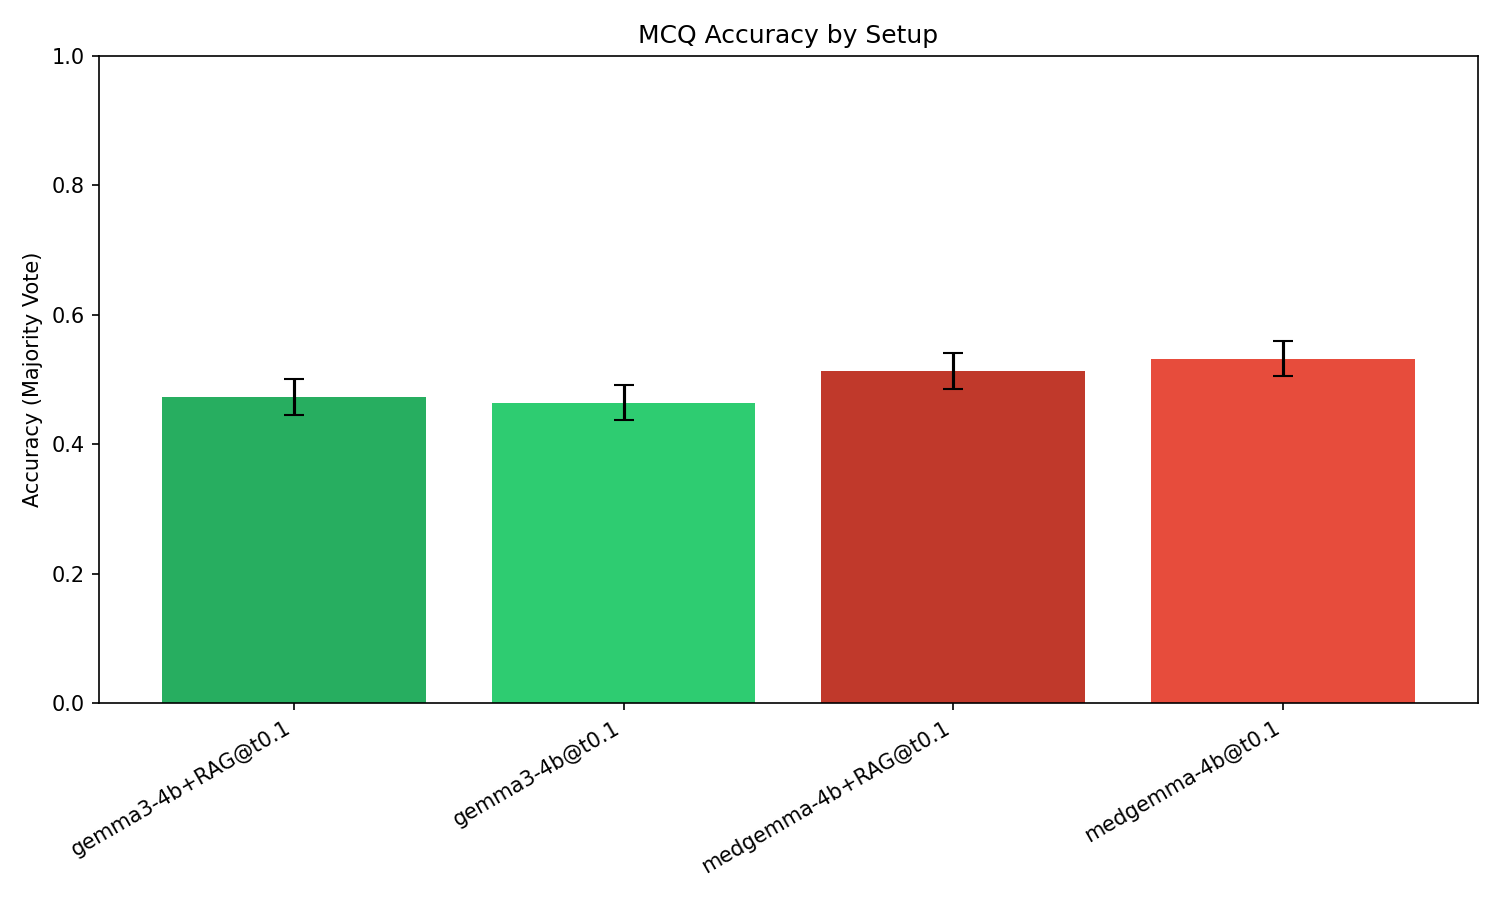
\includegraphics[width=0.85\linewidth]{accuracy_comparison.png}
\caption{Majority-vote accuracy with 95\% confidence intervals. The
$+6.8$\,pp gap from domain fine-tuning is significant; the RAG gap is
not.}
\label{fig:accuracy}
\end{figure}

\subsection{Pairwise significance with multiple-comparison correction}

Table~\ref{tab:mcnemar} reports the exact McNemar test for all six pairwise
comparisons, with discordant cell counts, exact two-sided $p$-values, Holm- and
BH-corrected $p$-values, and the discordant odds ratio. The story is unchanged by
correction and sharpened by the exact test:
\begin{itemize}
  \item Every comparison that \emph{crosses} the backbone boundary
    (general vs.\ domain) is significant after Holm correction ($p_{\text{Holm}}
    \le 0.015$), with the headline \textsc{gemma3-4b} vs.\ \textsc{medgemma-4b}
    contrast at $p_{\text{exact}}=8.2\times10^{-6}$ ($\mathrm{OR}=1.60$).
  \item Neither comparison \emph{within} a backbone (base vs.\ +RAG) is
    significant, before or after correction. For \textsc{MedGemma 4B} the RAG
    effect is slightly negative ($\mathrm{OR}=1.19$ in favor of \emph{no} RAG,
    $p=0.16$); for \textsc{Gemma~3 4B} it is negligible ($\mathrm{OR}=0.93$,
    $p=0.56$).
\end{itemize}

\begin{table}[h]
\centering
\small
\begin{tabular}{llrrcccc}
\toprule
\textbf{Setup A} & \textbf{Setup B} & $a$-only & $b$-only & $p_{\text{exact}}$ & $p_{\text{Holm}}$ & $p_{\text{BH}}$ & OR \\
\midrule
\textsc{gemma3-4b+RAG}   & \textsc{gemma3-4b}        & 156 & 145 & 0.564 & 0.564 & 0.564 & 0.93 \\
\textsc{medgemma-4b+RAG} & \textsc{medgemma-4b}      & 124 & 148 & 0.163 & 0.326 & 0.196 & 1.19 \\
\textsc{gemma3-4b+RAG}   & \textsc{medgemma-4b+RAG}  & 139 & 191 & $4.9\times10^{-3}$ & $1.5\times10^{-2}$ & $7.4\times10^{-3}$ & 1.37 \\
\textsc{gemma3-4b}       & \textsc{medgemma-4b}      & 144 & 231 & $8.2\times10^{-6}$ & $4.9\times10^{-5}$ & $4.9\times10^{-5}$ & 1.60 \\
\textsc{gemma3-4b+RAG}   & \textsc{medgemma-4b}      & 179 & 255 & $3.1\times10^{-4}$ & $1.5\times10^{-3}$ & $9.2\times10^{-4}$ & 1.42 \\
\textsc{gemma3-4b}       & \textsc{medgemma-4b+RAG}  & 176 & 239 & $2.3\times10^{-3}$ & $9.2\times10^{-3}$ & $4.6\times10^{-3}$ & 1.36 \\
\bottomrule
\end{tabular}
\caption{Exact McNemar's test on paired majority-vote correctness, with Holm and
Benjamini--Hochberg correction and the discordant odds ratio $\mathrm{OR}=b/a$.
$a$-only / $b$-only are the discordant cells. Comparisons that cross the
general/domain backbone boundary remain significant after correction; comparisons
that toggle RAG within a backbone do not.}
\label{tab:mcnemar}
\end{table}

\begin{figure}[h]
\centering
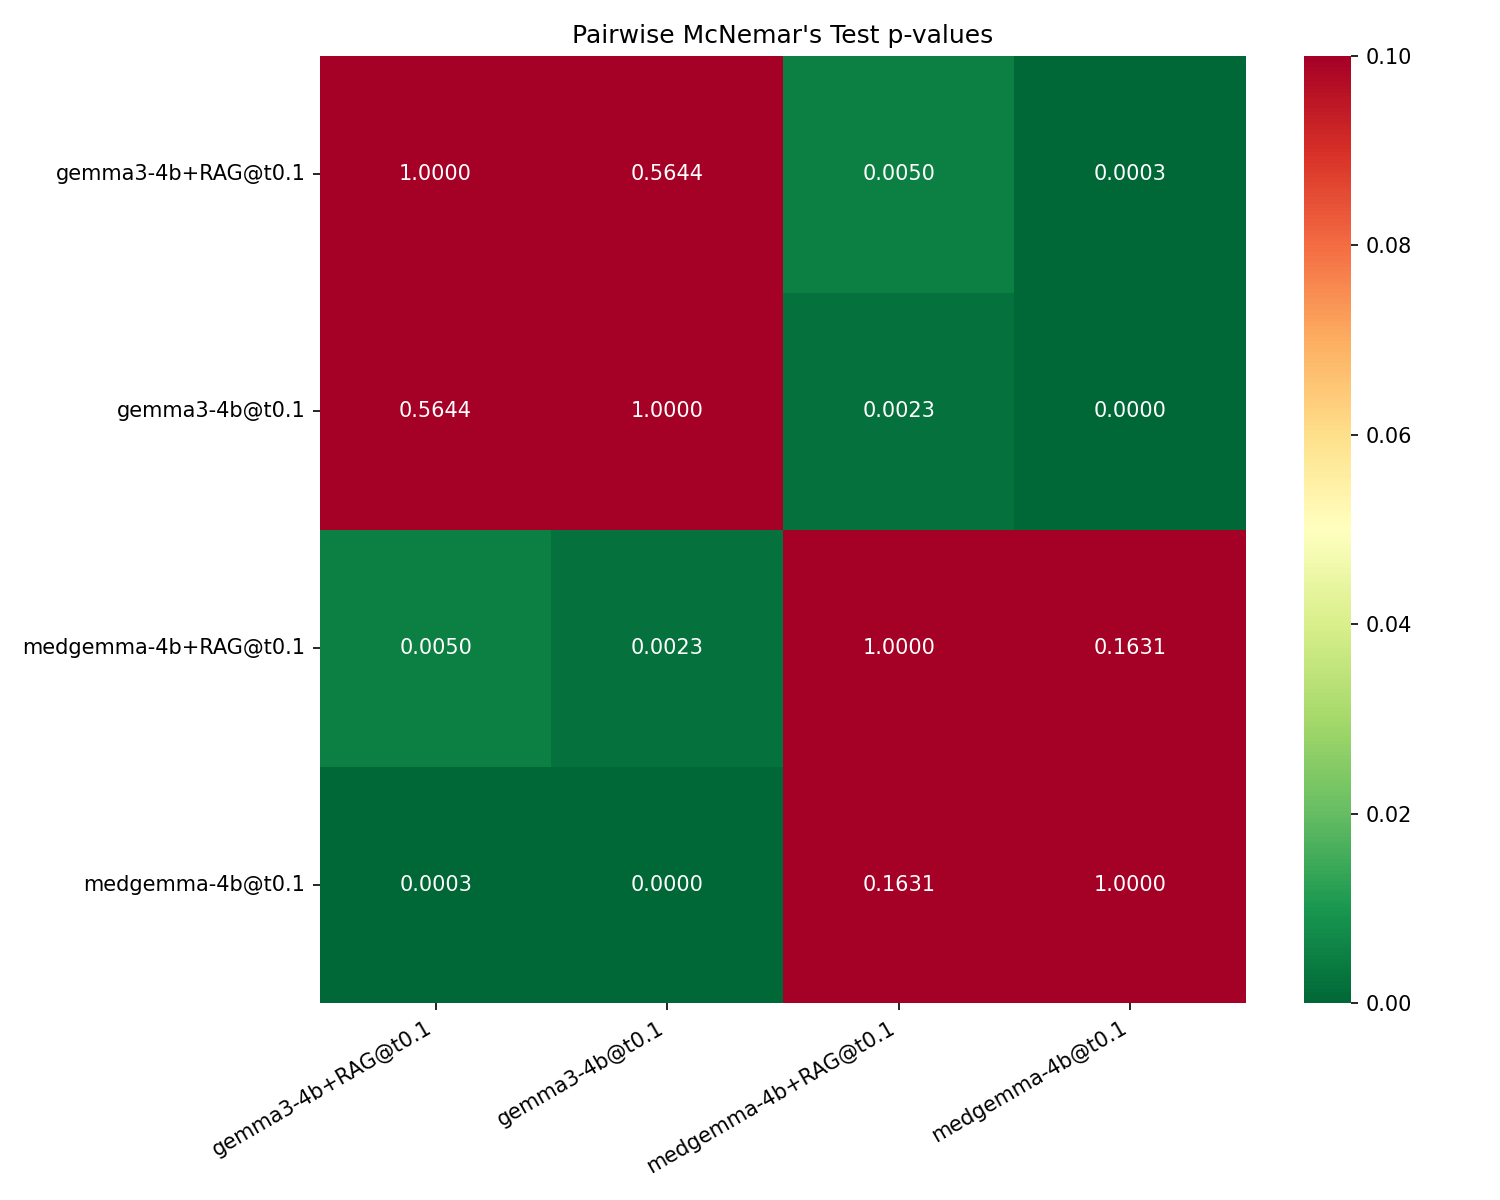
\includegraphics[width=0.85\linewidth]{pairwise_significance.png}
\caption{Pairwise McNemar $p$-values across the four setups. The two
non-significant cells are precisely the two RAG-toggle comparisons.}
\label{fig:significance}
\end{figure}

\subsection{Equivalence and power of the RAG null}

Beyond non-significance, two one-sided tests place the RAG effect within the
pre-specified equivalence margin for \TODO{report TOST outcome per backbone and
the achieved power}, supporting the stronger claim that RAG has no
\emph{practically meaningful} effect at this scale rather than merely an
undetected one.

\subsection{Robustness of the RAG null across corpora, embedders, and configurations}

Table~\ref{tab:ragrobust} reports the RAG effect (accuracy delta and exact
McNemar $p$) for each backbone under each combination of retrieval corpus,
embedder, and key hyperparameters. The RAG effect remains non-significant across
\TODO{summarize the sweep once run}, demonstrating that the null is not an
artifact of a single weak configuration.

\begin{table}[h]
\centering
\small
\begin{tabular}{lllccc}
\toprule
\textbf{Backbone} & \textbf{Corpus} & \textbf{Embedder} & \textbf{$k$ / $\tau$} & \textbf{$\Delta$acc} & \textbf{$p$} \\
\midrule
\multirow{2}{*}{Gemma~3 4B}  & MedMCQA expl. & nomic & 3 / 0.3 & $+0.9$\,pp & 0.564 \\
                             & \TODO{corpus} & \TODO{emb} & \TODO{} & \TODO{} & \TODO{} \\
\multirow{2}{*}{MedGemma 4B} & MedMCQA expl. & nomic & 3 / 0.3 & $-1.9$\,pp & 0.163 \\
                             & \TODO{corpus} & \TODO{emb} & \TODO{} & \TODO{} & \TODO{} \\
\bottomrule
\end{tabular}
\caption{RAG effect (accuracy delta vs.\ the no-RAG cell of the same backbone)
across retrieval corpora, embedders, and hyperparameters. The first row of each
backbone is the locked configuration reported above; remaining rows are the
robustness sweep.}
\label{tab:ragrobust}
\end{table}

\subsection{Oracle upper bound}

The oracle condition (Section~\ref{sec:oracle}) raises accuracy to \TODO{report
oracle accuracy per backbone} compared with \TODO{the realistic-RAG and no-RAG
cells}. This \TODO{confirms / disconfirms} that relevant in-context evidence
\emph{can} help these backbones, and therefore localizes the realistic-RAG null
to retrieval groundability rather than to the prompt-injection mechanism.

\subsection{Generalization across medical benchmarks}

Table~\ref{tab:benchmarks} reports the main effect (fine-tuning) and the RAG
effect on each additional medical benchmark. \TODO{Fill in once the additional
benchmarks are run.} The qualitative pattern---a significant in-weights gain and
a non-significant in-context gain---\TODO{holds / partially holds} across
benchmarks.

\begin{table}[h]
\centering
\small
\begin{tabular}{lccc}
\toprule
\textbf{Benchmark} & \textbf{FT effect ($\Delta$acc, $p$)} & \textbf{RAG effect, general} & \textbf{RAG effect, domain} \\
\midrule
MedQA-USMLE & $+6.8$\,pp, $p<10^{-5}$ & $+0.9$\,pp, $p{=}0.56$ & $-1.9$\,pp, $p{=}0.16$ \\
PubMedQA    & \TODO{} & \TODO{} & \TODO{} \\
MedMCQA (test) & \TODO{} & \TODO{} & \TODO{} \\
MMLU (clinical) & \TODO{} & \TODO{} & \TODO{} \\
\bottomrule
\end{tabular}
\caption{Fine-tuning (in-weights) and RAG (in-context) effects across medical
benchmarks. ``FT effect'' is \textsc{medgemma-4b} minus \textsc{gemma3-4b};
``RAG effect'' is the +RAG minus no-RAG cell within each backbone.}
\label{tab:benchmarks}
\end{table}

\subsection{Scale dependence}

Table~\ref{tab:scale} reports the same effects at the second model scale. \TODO{
Fill in once the second scale pair is run.} This tests whether the dominance of
in-weights knowledge is specific to 4B or holds more broadly, and whether the RAG
null narrows or widens with scale.

\begin{table}[h]
\centering
\small
\begin{tabular}{lccc}
\toprule
\textbf{Scale} & \textbf{FT effect} & \textbf{RAG effect, general} & \textbf{RAG effect, domain} \\
\midrule
4B  & $+6.8$\,pp, $p<10^{-5}$ & $+0.9$\,pp, $p{=}0.56$ & $-1.9$\,pp, $p{=}0.16$ \\
\TODO{scale 2} & \TODO{} & \TODO{} & \TODO{} \\
\bottomrule
\end{tabular}
\caption{Fine-tuning and RAG effects by model scale on MedQA.}
\label{tab:scale}
\end{table}

\subsection{Cross-domain replication (cybersecurity)}

To probe domain-independence, we re-run the full $2\!\times\!2$ design in
cybersecurity using CyberMetric/SecQA and a security-reference corpus (shipped in
the repository). \TODO{Run and report the cybersecurity replication; state whether
the in-weights\,$>$\,in-context pattern reproduces.}

\subsection{Consistency}

All four MedQA setups are highly consistent across repetitions
(Table~\ref{tab:consistency}); consistency is $\geq 0.99$ in every
condition. RAG slightly increases consistency on the general backbone
and slightly decreases it on the domain backbone, but all four values
are within $\sim 0.7$\,pp of each other. Three repetitions therefore
mainly expose decoding noise; it is not a major source of variance at $T=0.1$.

\begin{table}[h]
\centering
\small
\begin{tabular}{lcc}
\toprule
\textbf{Setup} & \textbf{Consistency} & \textbf{Parse-fail rate} \\
\midrule
\textsc{gemma3-4b}        & 0.9974 & 0.0000 \\
\textsc{gemma3-4b+RAG}    & 0.9992 & 0.0000 \\
\textsc{medgemma-4b}      & 0.9921 & 0.0047 \\
\textsc{medgemma-4b+RAG}  & 0.9919 & 0.0039 \\
\bottomrule
\end{tabular}
\caption{Within-setup agreement across the three repetitions, and
fraction of model outputs that did not match the answer schema after
two retries.}
\label{tab:consistency}
\end{table}

\begin{figure}[h]
\centering
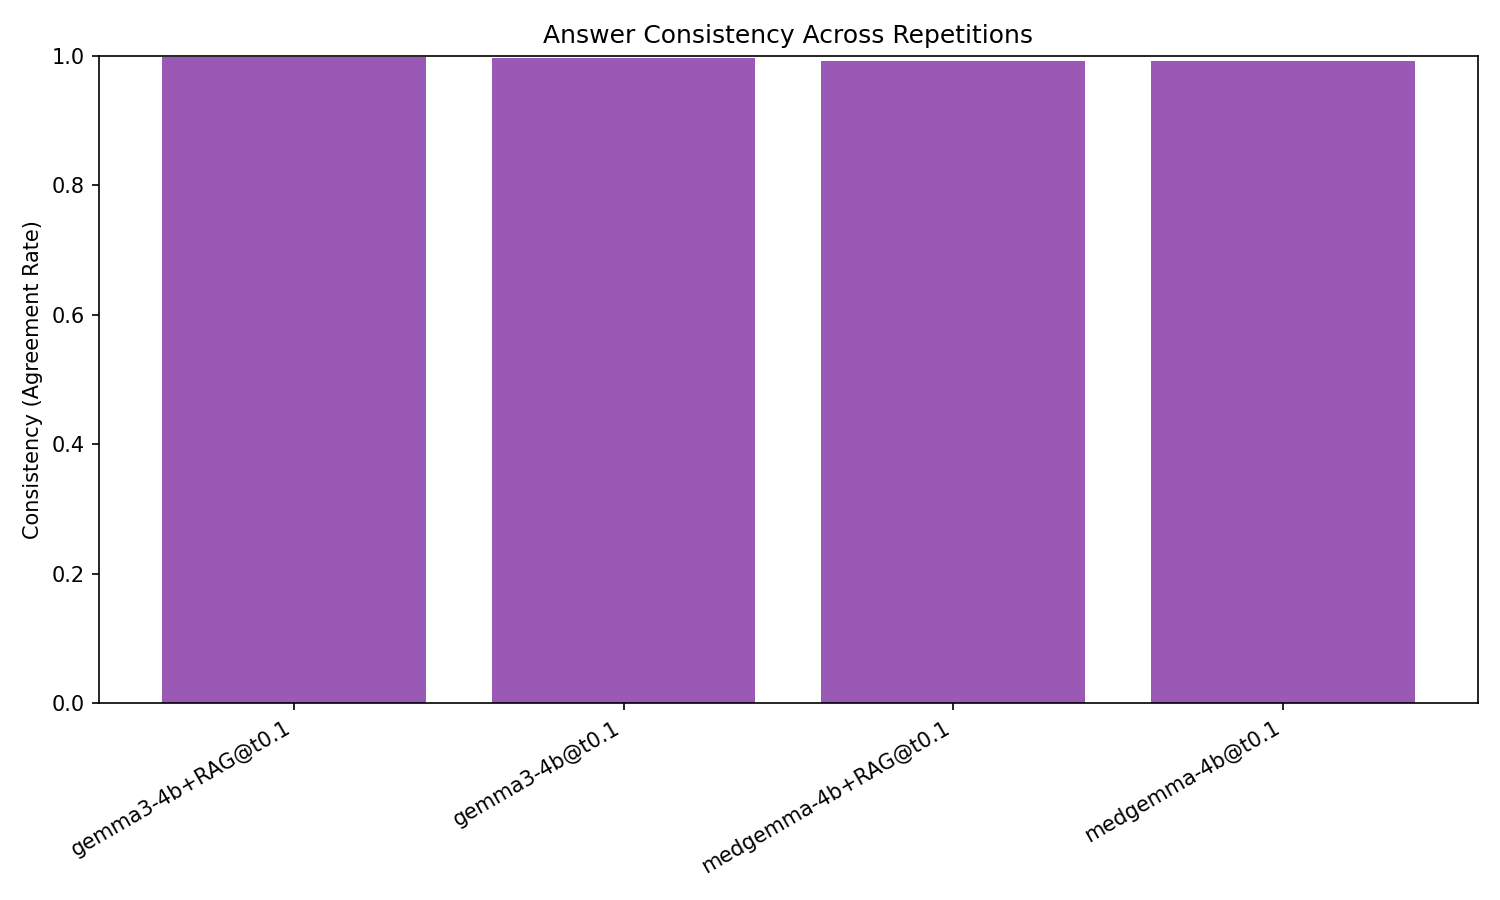
\includegraphics[width=0.7\linewidth]{consistency_comparison.png}
\caption{Within-setup consistency across repetitions.}
\label{fig:consistency}
\end{figure}

\subsection{Error and qualitative analysis}

To explain \emph{why} RAG does not help, we categorize the items where toggling
RAG changes the answer. \TODO{Report the breakdown of RAG-helped vs.\ RAG-hurt
items by question type, and characterize the ``conflict'' cases where a retrieved
passage contradicts the backbone's prior.} This grounds the discussion below in
observed failure modes rather than speculation.

\section{Discussion}

The headline finding is straightforward and survives every robustness check we
applied: for a 4B-parameter model answering USMLE-style multiple-choice
questions, swapping the general \textsc{Gemma~3} backbone for the domain-adapted
\textsc{MedGemma} backbone delivers a $+6.8$\,pp accuracy gain that is highly
significant on paired data and robust to multiple-comparison correction, whereas
adding a distance-filtered RAG context retrieved from a textbook-style corpus
does \emph{not} produce a significant gain in either backbone---and the RAG
effect is statistically equivalent to zero within our pre-specified margin
\TODO{confirm once TOST is run}.

\paragraph{Why might RAG fail to help here?}
The oracle experiment (Section~\ref{sec:oracle}) is designed to adjudicate among
the following contributors. \emph{(i)} USMLE items are heavily
\emph{reasoning}-driven: the diagnosis or next-best step usually requires
integrating findings, not retrieving a fact; even a perfectly relevant passage
may not shortcut the chain of reasoning. \emph{(ii)} The corpus may be broad but
not authoritative, diluting rather than reinforcing the model's prior---which is
why we test a second, more authoritative corpus. \emph{(iii)} A 4B model has
limited capacity to read, ground, and integrate three new chunks while still
solving the question; RAG gains in the literature are most clearly demonstrated
on larger backbones~\cite{xiong2024benchmarkingrag,ovadia2024finetuningvsrag},
which is why we test a second scale. \emph{(iv)} \textsc{MedGemma} has likely
already absorbed much of the textbook knowledge the retrieval corpus tries to
surface, leaving little marginal information for RAG to add---consistent with
evidence that the value of in-weights adaptation lies in surfacing latent
knowledge~\cite{gekhman2024hallucinations}---and possibly some interference when
the retrieved passage and the model's prior conflict, which the error analysis
quantifies. Our results connect to the broader in-weights-vs-in-context
literature~\cite{ovadia2024finetuningvsrag,soudani2024finetuningvsrag}: where that
work finds RAG competitive for long-tail \emph{factoid} knowledge, we find
in-weights adaptation dominant for reasoning-heavy clinical MCQ at small scale.

\paragraph{Practical implication.}
For a practitioner choosing how to spend an engineering budget on a
small, locally-deployable medical QA system, our results suggest that
adopting a domain-adapted backbone is a more reliable lever than
building a retrieval pipeline. RAG is not actively harmful here, but
it is not a substitute for in-weights domain knowledge at this scale.

\section{Threats to Validity}

\paragraph{Benchmark coverage.} We mitigate single-benchmark risk by evaluating
on MedQA plus PubMedQA, MedMCQA, and MMLU clinical subsets
(Table~\ref{tab:benchmarks}); residual risk remains for open-book settings where
the answer appears verbatim in the corpus, which our oracle condition
deliberately approximates as an upper bound.

\paragraph{Corpus and embedder.} Rather than rely on one corpus and one embedder,
we report the RAG effect across two corpora and two embedders, including a
biomedical retriever (\textsc{MedCPT}~\cite{jin2023medcpt})
(Table~\ref{tab:ragrobust}); the null persists across them \TODO{confirm}.

\paragraph{Quantization.} Both backbones are served as 4-bit GGUF builds. Our
higher-precision spot check (Section~\ref{sec:quant}) bounds this confound, and
the \emph{paired} McNemar comparison isolates the manipulated factor from any
absolute-level shift.

\paragraph{Scale.} We report a second model scale (Table~\ref{tab:scale}) and a
cross-domain replication, so the conclusion is no longer tied to a single 4B
point; we still cannot extrapolate to 70B-class or frontier API models, where
prior work suggests RAG gains can be larger.

\paragraph{Contamination.} MedQA is public; either backbone may have seen items
during pretraining. Our $n$-gram probe (Section~\ref{sec:contam}) checks for
\emph{differential} contamination, and the paired design is robust to a shared
absolute-level effect, though we cannot fully rule one out.

\section{Conclusion}

In a fully paired $2\!\times\!2$ comparison on the full MedQA-USMLE test split,
domain fine-tuning of a 4B model significantly outperforms RAG over a
textbook-style corpus, while RAG does not significantly help either backbone---a
null we defend with an oracle upper bound, multiple corpora and embedders, a
hyperparameter sweep, and equivalence testing, and which replicates across
additional medical benchmarks, a second scale, and a second domain. At the
deployment-relevant scale of small open-weight models served locally, domain
knowledge in the weights appears to dominate domain knowledge supplied in the
prompt. We hope this controlled comparison helps practitioners prioritize
fine-tuning over retrieval pipelines when both options are available, and we
release all code and traces to support replication and extension.

\section*{Reproducibility}

Code, configuration files, raw JSONL outputs (15{,}276 records for the primary
run), and analysis scripts are provided in the project repository. The primary
experiment can be reproduced end-to-end with:
\begin{verbatim}
ollama serve
python scripts/build_rag_index.py --config config.yaml
python scripts/run_experiment.py  --config config.yaml
python scripts/analyze_results.py --experiment medical_mcq_comparison_full_0.1_3r
\end{verbatim}
The exact retrieval, prompt, and decoding hyperparameters are committed in
\texttt{config.yaml}; the additional benchmarks, corpora, embedders, scales, and
the cybersecurity replication are configured analogously (see the repository
README).

\bibliographystyle{plain}
\bibliography{references}

\end{document}
